\documentclass[24pt]{article} % 文字的基本大小為24pt
\usepackage[margin=2cm]{geometry} % 設置頁面的邊距為2cm
\usepackage{graphicx} % 用於插入圖片
\usepackage{fontspec} % 用於設置字體
\usepackage{xeCJK} % 加入中日韓語
\setCJKmainfont{Noto Serif CJK SC} % 設定文字樣式
\usepackage{setspace} % 設置文檔的行距 
\onehalfspacing % 設置了1.5倍的行距

\begin{document}
 \begin{center}
\Large \textbf{2. CHAPTER}\\

\Large \textbf{章節2}\\

\Large \textbf{THEORETICAL BACKGROUND}\\

\Large \textbf{理論背景}\\
 \end{center}
This chapter is a brief introduction to the different systems that deal with data production collection and processing around the concept of enhancing all aspects of production that are favored by the academic community as well as the current and future state of industry for which these systems should prove to be indispensable.\\

\textbf{本章簡要介紹了處理數據生產的不同系統收集和加工圍繞著加強生產各個方面的概念,即 受到學術界以及行業現狀和未來狀況的青睞這些系統應該被證明是不可或缺的。}\\

It is important to notice from this part that these are not completely separate information systems. They start from different perspectives and they try to solve different problems but because of broad definitions they unavoidably expand into each other. That represents a problem on its own since from the available literature it becomes difficult to pinpoint where the boundary of a system ends and another one starts.\\

 \textbf{從這一部分需要注意的是,這些並不是完全獨立的資訊系統。他們從不同的角度出發,他們試圖解決不同的問題,但是由於定義寬泛,它們不可避免地相互擴展。這代表了問題本身,因為從現有的文獻中很難確定在哪裡一個系統的邊界結束,另一個系統的邊界開始。}\\

The Odoo management software (that is a topic of this work) considers PLM mainly as a tool for tracking change and improvements, while other key characteristics of PLM, like the use of digital items (later detailed at section 2.1), is a base characteristic of the material requirements planning which is a tool utility that also dabbles into MES.\\

\textbf{Odoo管理軟體(這是本文的主題)主要將PLM視為用於跟蹤更改和改進的工具,而PLM 的其他關鍵特徵,如使用數字專案稍後在第 2.1 節中詳述)是該材料的基本特徵需求規劃,這是一個工具實用程式,也涉足 MES。}\\

\begin{center}
\Large \textbf{2.1. Product lifecycle management }\\

\Large \textbf{2.1 產品生命週期管理}\\
\end{center}
Any information produced by an individual or team is done by an empirical creative process. A task requires either previous knowledge/experience or it will be inevitably plagued by mistakes and corrections, which in turn generates said experience in exchange of time and resources. That experience is, traditionally, embedded in the human resource (employee) that produced the information in the first place.\\

\textbf{個人或團隊產生的任何資訊都是由經驗創意完成的過程。一項任務要麼需要先前的知識或經驗,要麼將不可避免地受到困擾通過錯誤和更正,這反過來又產生了上述經驗以換取時間,並且資源。傳統上,這種經驗嵌入到人力資源(員工)中首先產生了資訊。}\\

Product Life-Cycle Management (PLM) is an organizational process that aims to control the flow of information regarding all aspects of a product throughout its life-cycle. As one can imagine, this definition, and its broad scope, does not make understanding PLM any easier. The thing to focus on, for all purposes, is that PLM true value is in what concerns change.\\

\textbf{產品生命週期管理(PLM)是一個旨在控制的組織過程有關產品整個生命週期各個方面的資訊流。合二為一可以想像,這個定義及其廣泛的範圍並不能使理解 PLM 成為任何容易。無論出於何種目的,需要關注的是 PLM 的真正價值在於關注什麼改變。}\\

\begin{center}
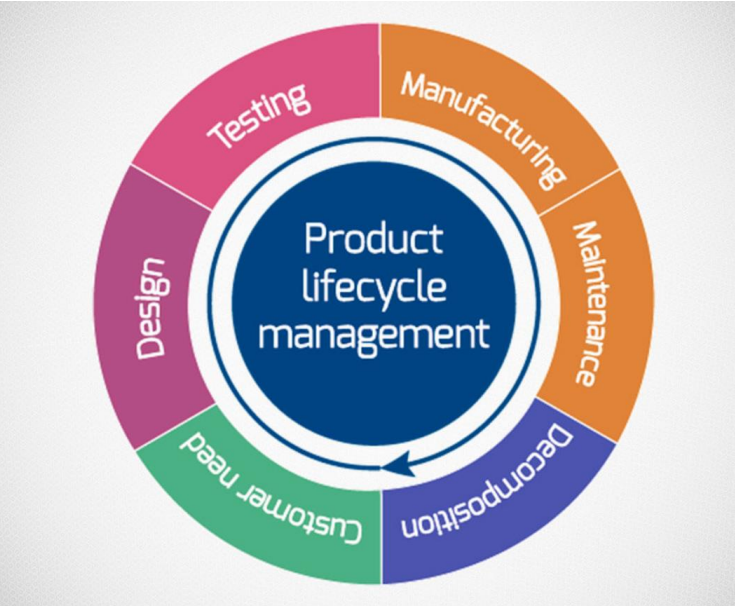
\includegraphics[width=15cm]{1.png}\\

Figure 1 Product lifecycle stages (Tripaldi, 2019)\\

圖1產品生命週期階段(Tripaldi,2019年)\\

\end{center}

PLM is above all a connecting technology, not an individual technology islet or information processing system (Saaksvuori and Immonen, 2008). The idea is that every information produced by company personnel holds value equivalent to the time and money invested. Using that information saves money, not using that information wastes money. This is easier to understand when looking to a design process.\\

\textbf{PLM首先是一種連接技術,而不是單個技術或信息處理系統(Saaksvuori和Immonen,2008)。這個想法是,每個公司人員提供的資訊具有相當於時間和金錢的價值 投資。使用這些資訊可以省錢,不使用這些資訊會浪費金錢。這在尋找設計過程時更容易理解。}\\

E.g. if an engineer designs an electronic circuit, the file holding the CAD drawing has an equivalent value to the time and money invested in it. The problem comes from the fact that in a traditional system only the engineer knows the design process behind the file, the extent of what is inside and its possible uses. While, from the perspective of the rest of the company, that is just a file in the database alongside thousands of others. The result is that, on its own, the information is of limited use.\\

\textbf{例如:如果工程師設計一個電子電路,則保存 CAD 圖紙的檔具有與投入的時間和金錢同等價值。問題來自以下事實在傳統系統中,只有工程師知道文件背後的設計過程,範圍裡面有什麼及其可能的用途。同時,從公司其他部門的角度來看,這隻是資料庫中的一個文件,還有數千個其他檔。結果是,就其本身而言,該資訊的用途有限。}\\

If by any chance there is another engineer working in a similar design it will become extremely difficult for him/her to find that file and use it in his own design. Ultimately this results in waste because Engineer*2 will have to spend more time and money doing something that was already made just because that information was not easily available or well organized.\\

\textbf{如果有另一位工程師從事類似的設計,它將成為他/她很難找到該檔並將其用於自己的設計。歸根結底,這導致浪費,因為工程師*2 將不得不花費更多的時間和金錢來做 僅僅因為該資訊不容易獲得而已經製作的東西,或者井井有條。}\\

This scenario is not limited to product design, but also to all aspects of the product lifecycle that produces change over time. Someone had to orchestrate how that piece will be produced , how that piece will be moved,packed , distributed and disposed of. When a problem is found or improvements are possible those changes also produce information and consume resources. If the company cannot take advantage of that existing information about all those phases of the product conception it will waste resources at every single redesign\\

\textbf{這個場景不僅限於產品設計,也涉及到產品的方方面面隨時間推移而產生變化的生命週期。必須有人來編排這件作品的樣子生產,該作品將如何移動、包裝、分發和處置。當 發現問題或可以改進,這些更改也會產生資訊和消耗資源。如果公司無法利用現有的資訊產品構思的所有這些階段都會在每次重新設計時浪費資源。}\\

Product Lifecycle Management consists of an information system that allows information and knowledge sharing within and between organizations (Sudarsan et al., 2005) minimizing the waste by controlling and organizing those files with information that would otherwise be carried only by the human resource that produced said files. The way it accomplishes that is by virtualizing all components of the product life-cycle in the form of digital “items” in an object oriented architecture. As explained by (Saaksvuori and Immonen, 2008),an item is a systematic and standard way to identify, encode and name a product, a product element or module, a component, a material or a service.\\

\textbf{產品生命週期管理由一個允許信息的信息系統組成以及組織內部和組織之間的知識共用(Sudarsan et al.,2005) 最小化通過控制和組織這些檔來浪費這些資訊,否則會 僅由生成所述檔的人力資源攜帶。它實現這一目標的方式是通過以數位“專案”的形式虛擬化產品生命週期的所有元件面向物件的架構。正如(Saaksvuori 和 Immonen,2008 年)所解釋的那樣,一個專案是一個 識別、編碼和命名產品、產品元素或產品的系統和標準方法模組、元件、材料或服務。}\\

These item objects are, by all means, virtual representations that hold metadata regarding what it tries to represent and allows to connect and link the information. As described by (D’Antonio et al., 2015) product information should be connected to its production process. PLM allows to link defined processes to the product and to provide constraints on the order of process execution. E.g. a CAD drawing for a circuit schematic is attached to a virtual circuit object that holds basic information about what is contained in the file and all the previous iterations of that file over time as well as links to items representing which bill of materials (BOM) it belongs to, the machines necessary to manufacture it, the processes necessary to assemble it and more importantly how all those items changed over each improving iteration.\\

\textbf{無論如何,這些項目物件都是虛擬表示形式,用於保存有關它試圖表示什麼,並允許連接和鏈接資訊。如(D'Antonio等人,2015)產品資訊應與其生產過程相關聯。 PLM 允許將定義的流程連結到產品,並對訂單提供約束的進程執行。例如:將電路原理圖的 CAD 圖紙附加到虛擬 circuit 物件,該物件保存有關檔中包含的內容的基本資訊以及所有該文件隨時間推移的先前反覆運算,以及指向表示哪個帳單的項目的連結它所屬的材料(BOM)、製造它所需的機器、工藝 組裝它所必需的,更重要的是所有這些專案在每個專案上是如何變化的改進反覆運算。}\\

This all-around virtualization gives precious context to information otherwise lost on its own complexity. It allows for faster access, easier understanding of the whole and the consequences of what happens when there is change for each part. This is the best way of organizing the existing data for future reference because it allows for structure as well as
transparency.\\

\textbf{這種全方位的虛擬化為資訊提供了寶貴的上下文,否則會丟失。自身的複雜性。它允許更快的訪問,更容易理解整體和當每個部分發生變化時會發生什麼後果。這是最好的方法組織現有數據以供將來參考,因為它允許結構和透明度。}\\

To sum up, PLM as a system aims to track functional change in all aspects regarding the product life, in a way that the company can benefit strategically from it by avoiding
informational waste. It does so by virtualizing the real thing in the form of digital items that store the files regarding what the item is supposed to represent. These can in turn be
correlated and tracked over time using metadata.\\

\textbf{總而言之,PLM 作為一個系統旨在跟蹤有關產品壽命,公司可以通過避免從中戰略性地受益資訊浪費。它通過以數字專案的形式虛擬化真實事物來做到這一點,這些數位專案存儲了有關項目應該代表什麼的檔。這些反過來可以是使用元數據隨時間推移進行關聯和追蹤。}\\

\begin{center}
\Large \textbf{2.2. Enterprise Resource Planing}\\

\Large \textbf{2.2 企業資源規劃}\\
\end{center}
In the early days of information systems, one of the first systems to find wide implementation was the called MRP (Material Requirements Planning). Although not necessarily software based, this system wide implementation was a natural consequence of computing technology and it aimed to solve bottlenecks regarding the material supplying and
product output by calculating the material needs for production. As it became more ubiquitous in the enterprise in the late 70’s and early 80’s the system evolved. This gave
origin to MRP II (Manufacturing Resource Planning) and, more important to the scope of this paper, ERP (Enterprise Resource Planning).\\

\textbf{在信息系統的早期,最早發現廣泛的系統之一實施稱為MRP(物料需求計劃)。雖然不是這種系統範圍的實現必然是基於軟體的,是計算技術,旨在解決材料供應和通過計算生產所需的材料來輸出產品。隨著它變得越來越多在70年代末和80年代初,該系統在企業中無處不在,並不斷發展。這給了起源於MRP II(製造資源規劃),更重要的是本文(ERP企業資源規劃)。}\\

For the most part modern Enterprise Resource Planning expands the original MRP function to encompass many other aspects of enterprise operations all while adding modularity to the system.\\

\textbf{在大多數情況下,現代企業資源規劃擴展了原來的物料需求計劃功能涵蓋企業運營的許多其他方面,同時添加系統的模組化。}\\

Modern ERP systems are often module based; different modules have different user interfaces and different user groups. For example, Manufacturing module, Procurement module, Logistics module, Financial module, Maintenance module, Sales module. (Saaksvuori and Immonen, 2008). These modules expand across many domains of knowledge but for the most part they do so always from the perspective of Production, Sales and Service. Figure 2 depicts the scope of the ERP system in comparison to other Information systems.\\

\textbf{現代ERP系統通常是基於模組的;不同的模組有不同的使用者介面和不同的使用者組。例如:「製造模組」、“採購” 模組、物流模組、財務模組、維護模組、銷售模組。 (Saaksvuori 和 Immonen,2008 年)。這些模組擴展到許多領域知識,但在大多數情況下,他們總是從生產、銷售的角度來這樣做和服務。圖2描述了ERP系統與其他資訊系統的比較範圍系統。}\\

\begin{center}
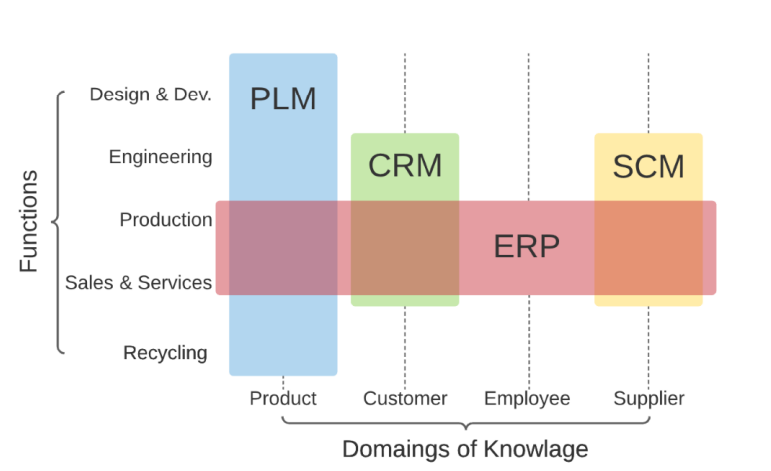
\includegraphics[width=15cm]{2.png}\\

Figure 2 Visual representation of the scope of different information systems (Adapted from Stark 2015)\\

圖2不同資訊系統範圍的可視化表示(改編自Stark 2015\\

\end{center}

This sort broad reach across the domains makes sense because the ERP operations, as were in the case of MRP, focus on handling transactions and orders. The focus of the ERP is controlling the change in input, retention and output of resources to the company, be of products, raw materials or packing.\\

\textbf{這種跨領域的廣泛覆蓋是有道理的,因為ERP操作,如在MRP的情況下,專注於處理交易和訂單。ERP的重點是控制對公司的資源投入、保留和產出的變化,包括產品、原材料或包裝。}\\

From the same image, it is possible to see the theoretical contrast between PLM and ERP even though they are both extremely broad. While ERP expands across the domains of knowledge but limits itself to a few functions, PLM expands across all functions that involve the product. As portrayed by Figure 3, another point of view that represents a good difference between the two is the lack of overlap in what concerns the scale or level of detail in which ERP and PLM affects the industry (i.e. the granularity of the two systems).\\

\textbf{從同一張圖片中,可以看出PLM和ERP之間的理論對比儘管它們都非常廣泛。雖然ERP擴展到以下領域知識,但僅限於少數功能,PLM 擴展到涉及的所有功能產品。如圖3所示,另一個觀點代表了一個很好的差異兩者之間在涉及規模或詳細程度方面缺乏重疊ERP和PLM影響著整個行業(即兩個系統的粒度)。}\\

\begin{center}
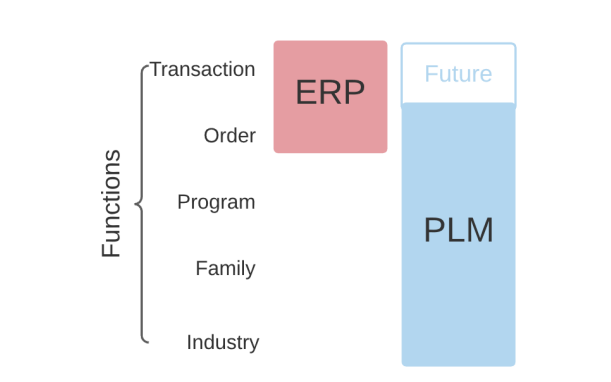
\includegraphics[width=15cm]{3.png}\\

Figure 3 Visual comparison of ERP and PLM concerning granularity (Adapted from Stark, 2015) \\

圖3 ERP和PLM在粒度上的直觀對比(改編自Stark,2015年)\\

\end{center}

As we can see, ERP is primarily concerned with the transaction and the order. Once an order is closed out, the ERP system processes the transactions with respect to that order but is not very much concerned with the order beyond that. On the other hand, PLM’s granularity is concerned with the order for the product and extends not only into the program, but into the family and the entire industry (Stark, 2015).\\

\textbf{正如我們所看到的,ERP主要關注交易和訂單。一次訂單被關閉,ERP系統處理與該訂單相關的交易,但除此之外,他不太關心訂單。另一方面,PLM 的粒度關注產品的訂單,不僅延伸到程式中,而且延伸到家庭和整個行業(Stark,2015)。}\\

This is particularly interesting because it demonstrates how the two systems can and do complement each other in the field. One of the aspects of ERP that should point out is that it is comparatively easier to integrate with other systems. ERP-MES integration for instance has been widely studied and implemented to the point where standards have been developed for it (ISA 95 - IEC 62264). One argument for this is the modular nature of the ERP system which is discussed further in the paper in (Chapter 5) with the analysis of the Odoo software. That is because the Odoo software evolved originally from an open-source ERP system.\\

\textbf{這特別有趣,因為它演示了這兩個系統如何能夠和執行在該領域相輔相成。ERP應該指出的一個方面是,它與其他系統集成相對容易。例如ERP-MES集成已被廣泛研究和實施,直到制定了標準(ISA 95 - IEC 62264)。其中一個論點是ERP系統的模組化性質在論文(第5章)中進一步討論了Odoo軟體。這是因為Odoo軟體最初是從開源ERP系統演變而來的。}\\

The nature of the ERP system is best summed up by (Umble et al. 2003): ERP provides a unified enterprise view of the business which encompasses all functions and departments, and an enterprise database in which all actions concerning finance, sales, marketing, purchasing and human resources are traced. The aim of this achieving is to expand the customers target and increase customers share in a market that slowly pivots to innovation (Vásquez and Escribano, 2017). \\

\textbf{ERP系統的本質最好地總結為(Umble et al. 2003):ERP提供了一個統一的企業業務視圖,包括所有職能和部門,以及一個企業資料庫,其中包含與財務、銷售、行銷、 採購和人力資源被追蹤。這一實現的目的是擴大客戶瞄準並增加客戶在緩慢轉向創新的市場中的份額(Vásquez 和 Escribano,2017年)。}\\

\begin{center}
\Large \textbf{2.3.  Manufacturing Execution System}\\

\Large \textbf{2.3 製造執行系統}\\
\end{center}
The final key of a fully integrated system would be the Manufacturing Execution System (MES). A MES is a layer of communication between the management and the production levels; it is a software that allows data exchange between the organizational level, usually supported by an ERP, and the shop-floor control systems, in which several, different, very customized software applications are employed (Meyer et al., 2009).\\

\textbf{一個完全集成的系統的最後一個關鍵是製造執行系統(MES)。MES是管理層和生產之間的溝通層水準;它是一種允許在組織級別之間進行數據交換的軟體,通常由ERP和車間控制系統支援,其中有幾個不同的,非常採用定製的軟體應用程式(Meyer 等人,2009 年)。}\\

Figure 4 is a nice depiction of how different systems fit within the scope of manufacturing and development.\\

\textbf{圖 4很好地描述了不同系統如何適應製造和開發範圍。}\\

\begin{center}
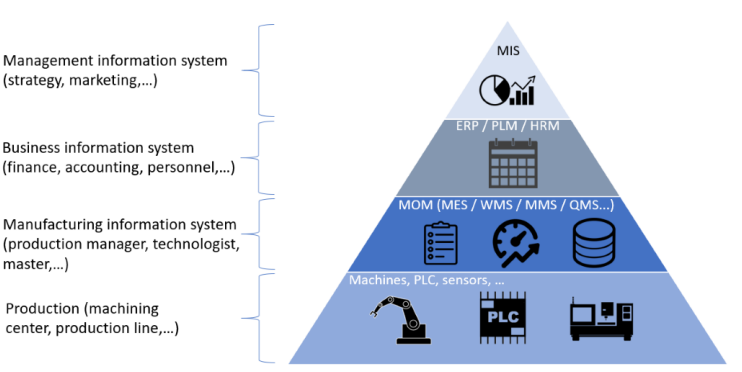
\includegraphics[width=15cm]{4.png}\\

Figure 4 Visual representation of the roll of different systems including MES (Adapted from mescenter.org)  \\

圖4 包括MES在內的不同系統的軋輥的可視化表示(改編自mescenter.org) \\

\end{center}

For all purposes MES main goal is to provide the numbers and data that ultimately is used to ascertain the condition and quality of not only the products but also all the processes that affect production. Machines, sensors, and anything that comes in contact with the product and provides output of any kind, basically, handing said data to the MES for sorting and processing in real time. E.g. if a manager wants to know the instant production numbers or to see a graphical representation of the rejection rate, that data will be available from a MES software.\\

\textbf{出於所有目的,MES的主要目標是提供最終使用的數位和數據不僅要確定產品的狀況和品質,還要確定所有過程影響生產。機器、感測器以及與產品接觸的任何東西並提供任何類型的輸出,基本上,將所述數據交給MES進行排序和實時處理。例如,如果經理想知道即時生產數位或要查看廢品率的圖形表示,該數據將從MES獲得軟體。}\\

Traditionally it is from this sort of information that management will evaluate efforts and make decisions. As mentioned before this sort of data collection fits perfectly to the use of ERP not only because the management of resources can be much more detailed if complemented by real time production data but also because the modularity of ERP usually means a seamless integration. MES (like ERP) has also been proven and implemented for decades and their implementation have already been standardized to a reasonable degree. \\

\textbf{傳統上,管理層將從此類資訊中評估努力和做出決定。如前所述,這種數據收集非常適合ERP不僅因為資源管理可以更加詳細,如果輔以即時生產數據,還因為ERP的模組化通常意味著無縫集成。MES(如ERP)也已被證明並實施幾十年來,它們的實施已經標準化到合理的程度。}\\

The functionalities of a MES have been grouped in 11 categories by MESA International (1997); furthermore, the tasks for each enterprise layer and, in turn, for each kind of information system are listed in the ISA95 – IEC62264 (2013) standard. This standard also provides definitions for the data structures to be exchanged among information systems aiming to enhance their integration; however, it mainly focuses on ERP-MES-Shop floor integration (D’Antonio et al., 2015).\\

\textbf{MES的功能被MESA International分為11個類別 (1997);此外,每個企業層的任務,以及每種信息系統列在ISA95 – IEC62264(2013)標準中。本標準還為資訊系統之間交換的數據結構提供定義旨在加強兩者的融合;但是,它主要集中在ERP-MES-車間 整合(D'Antonio等人,2015)。}\\

PLM studies by comparison are much more recent and PLM-MES integration, a main focus of this work, even more so. The challenge of this sort of integration and the state of the art regarding it was be covered in (Chapter 3) as well as the theoretical structure behind it. For now, suffice to point out that since MES provides the feedback by which changes are orchestrated and results are validated by generating information in the form of files and PLM focus on the tracking change by file organization there sure is value in the PLM-MES integration.\\

\textbf{相比之下,PLM 研究要新得多,而 PLM-MES 集成是主要的這項工作的重點,更是如此。這種整合的挑戰和(第3章)涵蓋了有關它的藝術以及它背後的理論結構。現在,只需指出,由於MES提供了更改的反饋通過以檔和 PLM 的形式生成資訊來編排和驗證結果專注於按文件組織跟蹤更改,PLM-MES肯定有價值集成。}\\

\begin{center}
\Large \textbf{2.4.  Industry 4.0}\\

\Large \textbf{2.4 工業4.0}\\
\end{center}
The term Industry 4.0 is one mentioned time and time again in modern literature as the next or current step in the evolution of production. It represents what is the 4th industrial revolution where the first was marked the adoption of steam power, the second was marked mainly using electrical power and the 3rd was characterized by the implementation of digital technology. Figure 5 nicely represents the progression of industrial revolutions.\\

\textbf{工業 4.0 一詞在現代文獻中一再被提及為生產演變的下一步或當前步驟。它代表什麼是4 TH工業革命,第一次標誌著蒸汽動力的採用,第二次標誌著主要使用電力和3 RD的特點是實施數位化科技。圖5很好地代表了工業革命的進展。}\\

\begin{center}
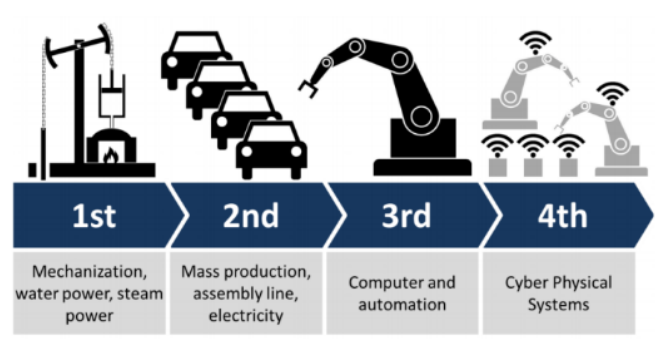
\includegraphics[width=15cm]{5.png}\\

Figure 5 The industry evolution (Adapted from STANCIOIU Alin, 2017)  \\

圖5行業演變(改編自STANCIOIU Alin,2017) \\

\end{center}

In broad strokes the 4th industrial revolution is (or will be) ultimately marked by the full integration between digital connectivity and production. As it is well known that the development of digital networks is the pivotal technology that sustain the modern world. It has changed the way humans interact and do business. However, whether the current level in which it is applied to the industry constitutes an industrial revolution is still uncertain because in all other revolutions have been marked by a violent increase in production that is yet to happen this time around. In fact, we are still to reach a shared definition of Industry 4.0.\\

\textbf{從廣義上講,第四次工業革命是(或將要)最終以數位連接與生產之間的集成。眾所周知,數位網路的發展是維持現代世界的關鍵技術。它改變了人類互動和做生意的方式。但是,當前水準是否在它應用於工業構成的工業革命仍然不確定,因為在所有其他革命中,都以生產的急劇增長為標誌,而這種增長尚未達到這一次發生。事實上,我們仍有待達成工業4.0的共同定義。}\\

What has been widely accepted however is that there are at least 3 technologies that characterize Industry 4.0. Those are the Internet of things (IoT), Cloud computing and the development of Cyber-Physical Systems (CPS), the last of which is particularly important for the context of this thesis.\\

\textbf{然而,被廣泛接受的是,至少有3種技術可以描述工業 4.0。這些是物聯網(IoT)、雲計算和開發資訊物理系統(CPS),其中最後一個尤為重要對於本論文的背景。}\\

CPS are systems consisting in a real entity (for example, a machine) and its corresponding virtual model – embedding all the models for mimicking the behavior of the real counterpart – capable to communicate with each other (D’Antonio et al., 2017). The idea is that, if one were to develop a digital twin (DT) of all physical instruments regarding a process in a system that allows for the digital counterparts to interact with each other as well as interacting with the physical world, innovation or change of said process would occur much faster and effectively. E.g., an engineer could simulate a change using the DT’s interaction, then, if successful, apply the change automatically to the production line in real time, execute tests, gather data and feed it back to the system without the need of manual input with all being done through the network.\\

\textbf{CPS 是由真實實體(例如機器)及其對應的實體組成的系統虛擬模型–嵌入所有模型以模仿真實模型的行為–能夠相互交流(D'Antonio 等人,2017年)。這個想法是,如果一個將開發有關系統中過程的所有物理儀器的數位孿生(DT)這允許數字對應物相互交互以及與物理世界,所述過程的創新或變化將發生得更快,並且有效。例如:工程師可以使用DT的交互來類比變化,然後如果成功,將變更自動即時應用到生產線上,執行測試,收集數據並將其反饋給系統,無需手動輸入通過網路完成。}\\

The main point to be derived from all this is that PLM-MES systems possibly are the first step to achieve a proper CPS since it provides for the virtualization and necessary control to reach something near a virtual twin. The debatable matter is how deep is its current effect in industrial application.\\

\textbf{從這一切中得出的要點是,PLM-MES系統可能是第一個步驟來實現適當的CPS,因為它提供了虛擬化和必要的控制到達虛擬孿生體附近的某物。值得商榷的問題是,它目前對工業應用的影響有多深工業應用。}\\

Nonetheless, the term Industry 4.0 is, if anything, a useful denotation to the increasing application of digital connectivity, network development and the internet to industry.\\

\textbf{儘管如此,工業4.0一詞,如果有的話,對日益增長的數位連接、網路發展和互聯網在工業中的應用。}\\

Another term often included within the scope of Industry 4.0 is the called Lot Size One or Lot 1. This is the idea of each item customized to the individual specifications of the buyer in a system in which a customer order does not start supply chain equipment moving; it turns on manufacturing machines. \\

\textbf{工業4.0範圍內通常包含的另一個術語稱為 Lot Size One 或拍品1.這是根據買方的個人化規格定製每件商品的想法在客戶訂單不啟動供應鏈設備行動的系統中;原來如此在製造機器上。}\\

The theory behind it is that as production and development becomes more and more flexible as this sort of manufacturing becomes not only viable but also attractive. Having a tailored requested product means that there are no storage requirements, no inventory overhead, and of course a 100 percent guaranteed sell. This concept is not new by any means, in fact it predates Industry 4.0 quite a lot. In the book “The machine that changed the world” the authors (Womack et al., 1990) discuss that toward this end, lean producers employ teams of multiskilled workers at all levels of the organization and use highly flexible, increasingly automated machines to produce volumes of products in enormous variety.\\

\textbf{其背後的理論是,隨著生產和發展變得越來越多靈活性,因為這種製造不僅可行而且具有吸引力。擁有量身定製的產品意味著沒有存儲要求,沒有庫存開銷,當然還有百分之100保證銷售。這個概念無論如何都不是新鮮事物,因為事實上,它早於工業 4.0。在《改變世界的機器》一書中作者(Womack et al.,1990)討論說,為此,精益生產者雇用了團隊在組織的各個層面使用高度靈活的多技能工人,越來越多地自動化機器可生產種類繁多的產品。}\\

In a way ‘Lot Size One’ is nothing more than the extrapolation of this sort of thinking. Of course, the industry is yet to reach such level of production flexibility, but glimpses of this sort of mentality can already be seem on more modular productions. One of the best examples is amazon packing systems. E.g. a customer receives a package from Amazon containing a mix of products that has been packaged just for him/her according to their specific order. Although superficial in nature, this represents a high level of customization for the customer.\\

\textbf{在某種程度上,“一手數”只不過是這種思維的外推。當然,該行業尚未達到這種生產靈活性水準,但可以一窺這一點 這種心態已經出現在更多的模組化產品上。最好的例子之一是亞馬遜包裝系統。例如,買家收到來自亞馬遜的包裹,其中包含根據特定順序為他/她包裝的產品群組。雖然本質上是膚淺的,但這代表了對客戶的高度定製。}\\

Another great example is electronics prototyping. Currently there are companies that take your printed circuit board designs and BOM, delivering small batches of assembled prototypes at a low cost. Prototyping of electronical devices used to be a highly expensive process, but some companies have flexibilized their production to the degree where they are able to deliver it fast and reliably. Again, that is possible because electronics components are inherently modular systems even if of high complexity. The following image (Figure 6 Example project of power supply adaptor circuit) is an example of an electronic circuit that was designed by this student and manufactured by JLCPCB within a single week.\\

\textbf{另一個很好的例子是電子原型設計。目前有公司採取您的印刷電路板設計和 BOM,提供小批量組裝的低成本的原型。電子設備的原型設計曾經非常昂貴過程,但一些公司已經將他們的生產靈活化到他們所處的程度能夠快速可靠地交付。同樣,這是可能的,因為電子元件是固有的模組化系統,即使複雜度很高。下圖(圖 6電源適配器電路的示例專案)是電子電路的一個例子由這位學生設計,並由JLCPCB在一周內製造。}\\

\begin{center}
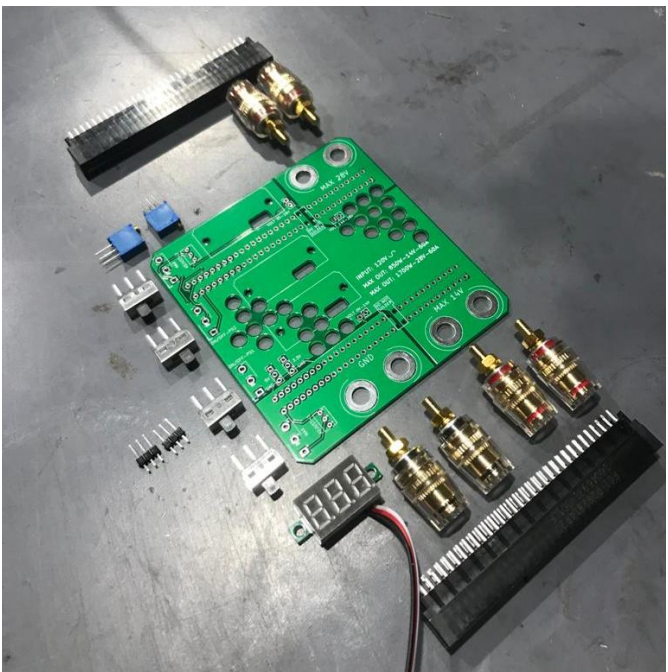
\includegraphics[width=15cm]{6.png}\\

Figure 6 Example project of power supply adaptor circuit   \\

圖6為電源配接器電路示例專案 \\

\end{center}

All and all, the result is again a greater need for control and management of change. Which means the implementation of a PLM-MES system would be of great help. PLM would be required to manage change and innovation throughout the lifecycle of small batch products and MES would provide the real time reaction and feedback necessary to reduce errors that could cause losing a whole batch. \\

\textbf{總而言之,其結果再次是對變革的控制和管理的更大需求。意味著PLM-MES系統的實施將有很大説明。PLM 將是需要在小批量產品的整個生命週期內管理變更和創新 MES將提供必要的即時反應和反饋,以減少錯誤可能會導致丟失一整批。}\\


\end{document}